% ============================================================
% DASK 2026 TWIN TOWERS - FLOOR PLAN
% TikZ Drawing with detailed annotations
% ============================================================
\documentclass[a4paper,12pt]{article}
\usepackage[utf8]{inputenc}
\usepackage[T1]{fontenc}
\usepackage{tikz}
\usepackage{pgfplots}
\pgfplotsset{compat=1.18}
\usepackage{geometry}
\geometry{margin=1.5cm}
\usepackage{siunitx}
\usepackage{amsmath}
\usepackage{xcolor}

\usetikzlibrary{patterns, arrows.meta, calc, positioning, decorations.pathreplacing}

% Define colors
\definecolor{shearwall}{RGB}{100,100,100}
\definecolor{column}{RGB}{50,50,50}
\definecolor{beam}{RGB}{0,100,200}
\definecolor{brace}{RGB}{200,100,0}
\definecolor{core}{RGB}{150,75,0}
\definecolor{tower1}{RGB}{70,130,180}
\definecolor{tower2}{RGB}{180,100,70}

\title{\textbf{DASK 2026 Twin Towers}\\Floor Plan \& Structural Layout}
\author{Structural Engineering Documentation}
\date{February 2026}

\begin{document}
\maketitle

% ============================================================
% SECTION 1: TYPICAL FLOOR PLAN
% ============================================================
\section{Typical Floor Plan (Top View)}

\begin{center}
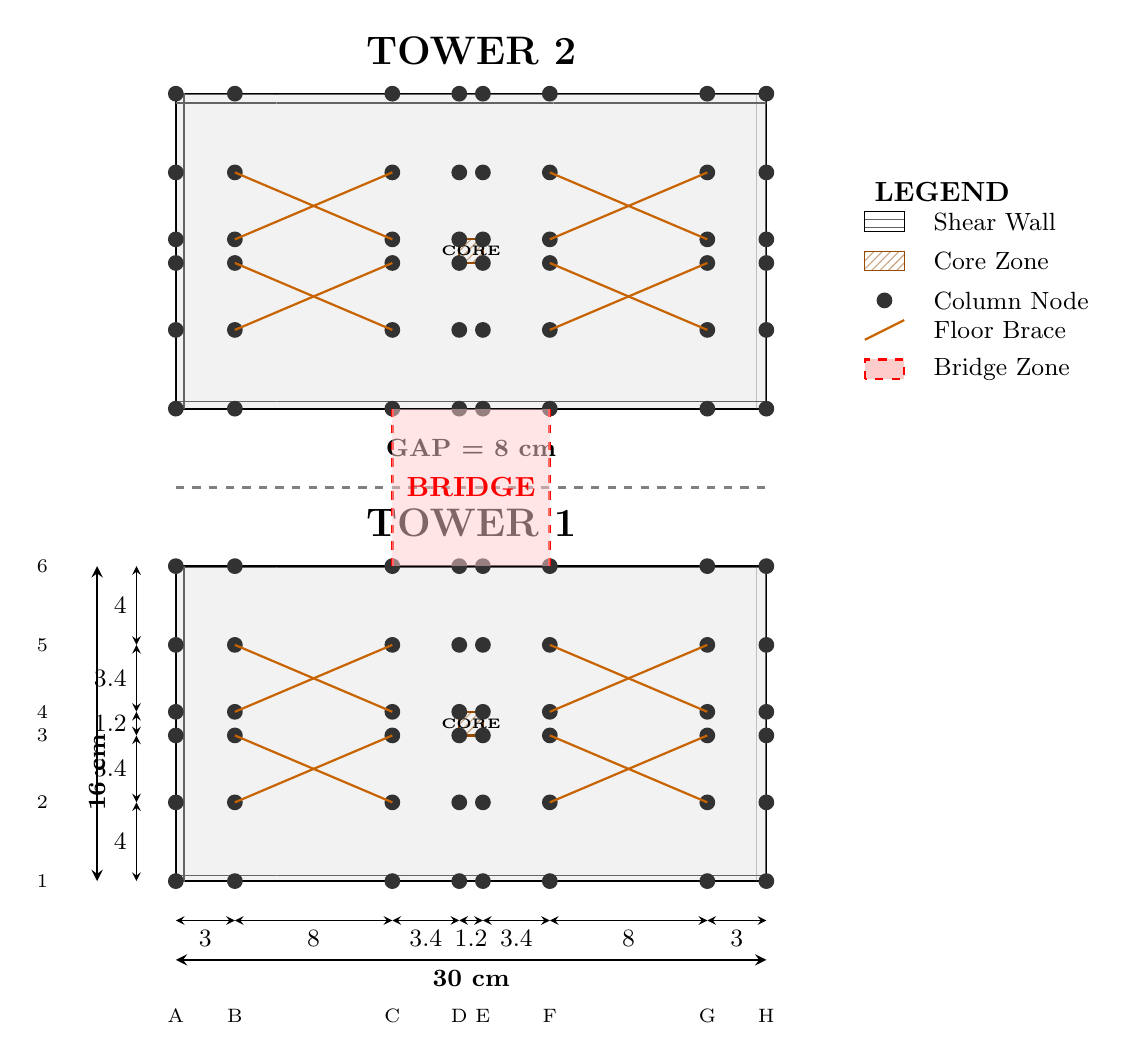
\begin{tikzpicture}[scale=0.25, font=\small]

    % -------------------------------------------------
    % TOWER 1 (Y = 0 to 16)
    % -------------------------------------------------
    \begin{scope}[shift={(0,0)}]
        % Grid coordinates
        % X: 0, 3, 11, 14.4, 15.6, 19, 27, 30
        % Y: 0, 4, 7.4, 8.6, 12, 16
        
        % Floor slab outline
        \draw[thick, fill=gray!10] (0,0) rectangle (30,16);
        
        % Core zone (hatched)
        \fill[pattern=north east lines, pattern color=core!50] 
            (14.4, 7.4) rectangle (15.6, 8.6);
        \draw[thick, core] (14.4, 7.4) rectangle (15.6, 8.6);
        \node at (15, 8) {\tiny\textbf{CORE}};
        
        % Shear walls on edges (hatched)
        % Front wall (Y=0)
        \fill[pattern=horizontal lines, pattern color=shearwall] 
            (0,0) rectangle (30,0.5);
        % Back wall (Y=16)
        \fill[pattern=horizontal lines, pattern color=shearwall] 
            (0,15.5) rectangle (30,16);
        % Left wall (X=0)
        \fill[pattern=vertical lines, pattern color=shearwall] 
            (0,0) rectangle (0.5,16);
        % Right wall (X=30)
        \fill[pattern=vertical lines, pattern color=shearwall] 
            (29.5,0) rectangle (30,16);
        
        % Column grid points
        \foreach \x in {0, 3, 11, 14.4, 15.6, 19, 27, 30} {
            \foreach \y in {0, 4, 7.4, 8.6, 12, 16} {
                \fill[column] (\x, \y) circle (0.4);
            }
        }
        
        % X-bracing pattern (floor diaphragm)
        \draw[brace, thick] (3,4) -- (11,7.4);
        \draw[brace, thick] (11,4) -- (3,7.4);
        \draw[brace, thick] (19,4) -- (27,7.4);
        \draw[brace, thick] (27,4) -- (19,7.4);
        \draw[brace, thick] (3,8.6) -- (11,12);
        \draw[brace, thick] (11,8.6) -- (3,12);
        \draw[brace, thick] (19,8.6) -- (27,12);
        \draw[brace, thick] (27,8.6) -- (19,12);
        
        % Dimension lines - X direction (bottom)
        \draw[<->, >=stealth] (0,-2) -- (3,-2) node[midway, below] {3};
        \draw[<->, >=stealth] (3,-2) -- (11,-2) node[midway, below] {8};
        \draw[<->, >=stealth] (11,-2) -- (14.4,-2) node[midway, below] {3.4};
        \draw[<->, >=stealth] (14.4,-2) -- (15.6,-2) node[midway, below] {1.2};
        \draw[<->, >=stealth] (15.6,-2) -- (19,-2) node[midway, below] {3.4};
        \draw[<->, >=stealth] (19,-2) -- (27,-2) node[midway, below] {8};
        \draw[<->, >=stealth] (27,-2) -- (30,-2) node[midway, below] {3};
        
        % Dimension lines - Y direction (left)
        \draw[<->, >=stealth] (-2,0) -- (-2,4) node[midway, left] {4};
        \draw[<->, >=stealth] (-2,4) -- (-2,7.4) node[midway, left] {3.4};
        \draw[<->, >=stealth] (-2,7.4) -- (-2,8.6) node[midway, left] {1.2};
        \draw[<->, >=stealth] (-2,8.6) -- (-2,12) node[midway, left] {3.4};
        \draw[<->, >=stealth] (-2,12) -- (-2,16) node[midway, left] {4};
        
        % Total dimensions
        \draw[<->, >=stealth, thick] (0,-4) -- (30,-4) node[midway, below] {\textbf{30 cm}};
        \draw[<->, >=stealth, thick] (-4,0) -- (-4,16) node[midway, left, rotate=90] {\textbf{16 cm}};
        
        % Label
        \node[above] at (15, 17) {\Large\textbf{TOWER 1}};
    \end{scope}
    
    % -------------------------------------------------
    % GAP BETWEEN TOWERS
    % -------------------------------------------------
    \draw[dashed, gray, thick] (0,20) -- (30,20);
    \draw[dashed, gray, thick] (0,24) -- (30,24);
    \node at (15, 22) {\textbf{GAP = 8 cm}};
    
    % -------------------------------------------------
    % TOWER 2 (Y = 24 to 40)
    % -------------------------------------------------
    \begin{scope}[shift={(0,24)}]
        % Floor slab outline
        \draw[thick, fill=gray!10] (0,0) rectangle (30,16);
        
        % Core zone (hatched)
        \fill[pattern=north east lines, pattern color=core!50] 
            (14.4, 7.4) rectangle (15.6, 8.6);
        \draw[thick, core] (14.4, 7.4) rectangle (15.6, 8.6);
        \node at (15, 8) {\tiny\textbf{CORE}};
        
        % Shear walls on edges (hatched)
        \fill[pattern=horizontal lines, pattern color=shearwall] 
            (0,0) rectangle (30,0.5);
        \fill[pattern=horizontal lines, pattern color=shearwall] 
            (0,15.5) rectangle (30,16);
        \fill[pattern=vertical lines, pattern color=shearwall] 
            (0,0) rectangle (0.5,16);
        \fill[pattern=vertical lines, pattern color=shearwall] 
            (29.5,0) rectangle (30,16);
        
        % Column grid points
        \foreach \x in {0, 3, 11, 14.4, 15.6, 19, 27, 30} {
            \foreach \y in {0, 4, 7.4, 8.6, 12, 16} {
                \fill[column] (\x, \y) circle (0.4);
            }
        }
        
        % X-bracing pattern
        \draw[brace, thick] (3,4) -- (11,7.4);
        \draw[brace, thick] (11,4) -- (3,7.4);
        \draw[brace, thick] (19,4) -- (27,7.4);
        \draw[brace, thick] (27,4) -- (19,7.4);
        \draw[brace, thick] (3,8.6) -- (11,12);
        \draw[brace, thick] (11,8.6) -- (3,12);
        \draw[brace, thick] (19,8.6) -- (27,12);
        \draw[brace, thick] (27,8.6) -- (19,12);
        
        % Label
        \node[above] at (15, 17) {\Large\textbf{TOWER 2}};
    \end{scope}
    
    % -------------------------------------------------
    % BRIDGE ZONES (indicated)
    % -------------------------------------------------
    \draw[very thick, red, dashed] (11, 16) -- (11, 24);
    \draw[very thick, red, dashed] (19, 16) -- (19, 24);
    \fill[red!20, opacity=0.5] (11, 16) rectangle (19, 24);
    \node[red, font=\bfseries] at (15, 20) {BRIDGE};
    
    % -------------------------------------------------
    % LEGEND
    % -------------------------------------------------
    \begin{scope}[shift={(35, 30)}]
        \node[anchor=west, font=\bfseries] at (0, 5) {LEGEND};
        
        % Shear wall
        \fill[pattern=horizontal lines, pattern color=shearwall] (0, 3) rectangle (2, 4);
        \draw (0, 3) rectangle (2, 4);
        \node[anchor=west] at (3, 3.5) {Shear Wall};
        
        % Core
        \fill[pattern=north east lines, pattern color=core!50] (0, 1) rectangle (2, 2);
        \draw[core] (0, 1) rectangle (2, 2);
        \node[anchor=west] at (3, 1.5) {Core Zone};
        
        % Column
        \fill[column] (1, -0.5) circle (0.4);
        \node[anchor=west] at (3, -0.5) {Column Node};
        
        % Brace
        \draw[brace, thick] (0, -2.5) -- (2, -1.5);
        \node[anchor=west] at (3, -2) {Floor Brace};
        
        % Bridge
        \fill[red!20] (0, -4.5) rectangle (2, -3.5);
        \draw[red, dashed, thick] (0, -4.5) rectangle (2, -3.5);
        \node[anchor=west] at (3, -4) {Bridge Zone};
    \end{scope}
    
    % -------------------------------------------------
    % GRID LABELS
    % -------------------------------------------------
    % X-axis labels
    \node[below] at (0, -6) {\scriptsize A};
    \node[below] at (3, -6) {\scriptsize B};
    \node[below] at (11, -6) {\scriptsize C};
    \node[below] at (14.4, -6) {\scriptsize D};
    \node[below] at (15.6, -6) {\scriptsize E};
    \node[below] at (19, -6) {\scriptsize F};
    \node[below] at (27, -6) {\scriptsize G};
    \node[below] at (30, -6) {\scriptsize H};
    
    % Y-axis labels (Tower 1)
    \node[left] at (-6, 0) {\scriptsize 1};
    \node[left] at (-6, 4) {\scriptsize 2};
    \node[left] at (-6, 7.4) {\scriptsize 3};
    \node[left] at (-6, 8.6) {\scriptsize 4};
    \node[left] at (-6, 12) {\scriptsize 5};
    \node[left] at (-6, 16) {\scriptsize 6};
    
\end{tikzpicture}
\end{center}

\vspace{1cm}

\section{Grid Coordinates}

\begin{center}
\begin{tabular}{|c|c|c|}
\hline
\textbf{Direction} & \textbf{Grid Lines} & \textbf{Spacing (cm)} \\
\hline
X-Direction & A, B, C, D, E, F, G, H & 3 - 8 - 3.4 - 1.2 - 3.4 - 8 - 3 \\
\hline
Y-Direction (per tower) & 1, 2, 3, 4, 5, 6 & 4 - 3.4 - 1.2 - 3.4 - 4 \\
\hline
\end{tabular}
\end{center}

\section{Structural Summary}

\begin{itemize}
    \item \textbf{Tower Dimensions:} $30 \times 16$ cm each
    \item \textbf{Gap Between Towers:} 8 cm
    \item \textbf{Total Footprint:} $30 \times 40$ cm
    \item \textbf{Core Zone:} $1.2 \times 1.2$ cm at center
    \item \textbf{Building Height:} 159 m (27 floors)
    \item \textbf{Fundamental Period:} $T_1 = 0.0608$ s
    \item \textbf{Weight:} 3.357 kg
\end{itemize}

\newpage

% ============================================================
% SECTION 2: ELEVATION VIEWS
% ============================================================
\section{Elevation Views}

% -------------------------------------------------
% FRONT VIEW (XZ Plane, Y=0)
% -------------------------------------------------
\subsection{Front Elevation (Y = 0)}

\begin{center}
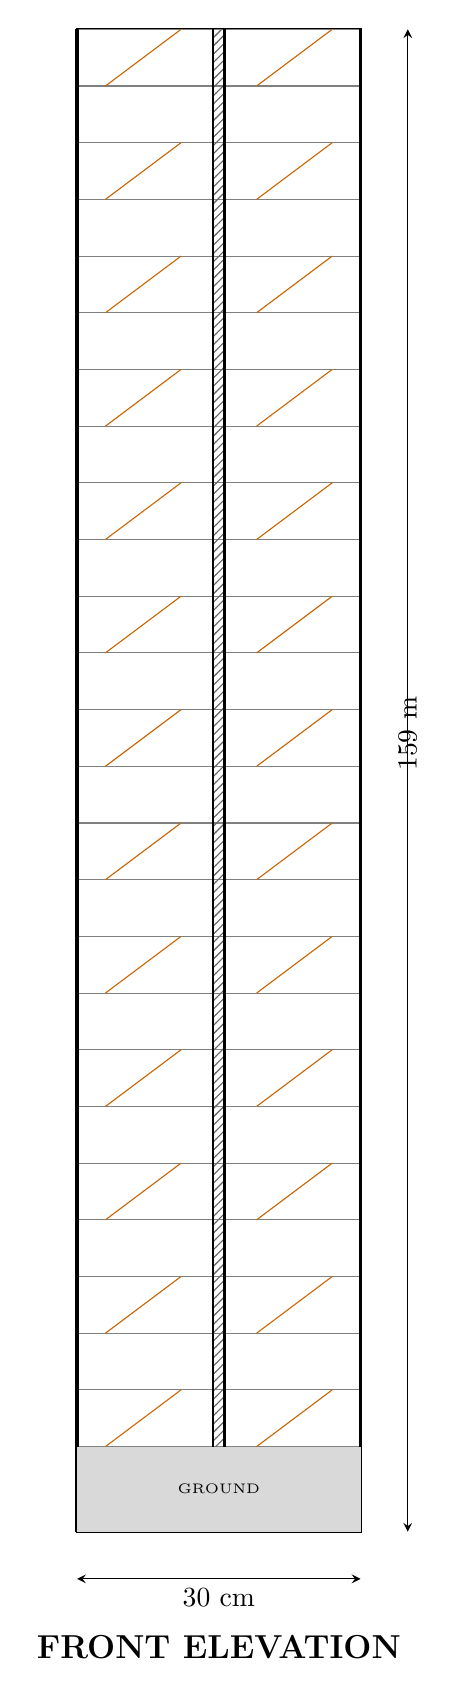
\begin{tikzpicture}[scale=0.12, font=\tiny]
    
    % Building outline
    \draw[thick] (0,0) rectangle (30, 159);
    
    % Floor lines
    \foreach \f in {0, 9, 15, 21, 27, 33, 39, 45, 51, 57, 63, 69, 75, 81, 87, 93, 99, 105, 111, 117, 123, 129, 135, 141, 147, 153, 159} {
        \draw[gray, thin] (0, \f) -- (30, \f);
    }
    
    % Shear walls at core (D-E zone, hatched)
    \fill[pattern=north east lines, pattern color=shearwall] 
        (14.4, 0) rectangle (15.6, 159);
    \draw[thick] (14.4, 0) -- (14.4, 159);
    \draw[thick] (15.6, 0) -- (15.6, 159);
    
    % Corner columns
    \draw[very thick] (0, 0) -- (0, 159);
    \draw[very thick] (30, 0) -- (30, 159);
    
    % DAMA bracing pattern (simplified)
    \foreach \f in {0, 2, 4, 6, 8, 10, 12, 14, 16, 18, 20, 22, 24} {
        \pgfmathsetmacro{\zbot}{\f * 6 + 9}
        \pgfmathsetmacro{\ztop}{\zbot + 6}
        % Alternating diagonals
        \pgfmathparse{mod(\f, 2) == 0 ? 1 : 0}
        \ifnum\pgfmathresult=1
            \draw[brace] (3, \zbot) -- (11, \ztop);
            \draw[brace] (19, \zbot) -- (27, \ztop);
        \else
            \draw[brace] (11, \zbot) -- (3, \ztop);
            \draw[brace] (27, \zbot) -- (19, \ztop);
        \fi
    }
    
    % Ground floor
    \fill[gray!30] (0, 0) rectangle (30, 9);
    \node at (15, 4.5) {GROUND};
    
    % Dimension
    \draw[<->, >=stealth] (0, -5) -- (30, -5) node[midway, below] {\normalsize 30 cm};
    \draw[<->, >=stealth] (35, 0) -- (35, 159) node[midway, right, rotate=90] {\normalsize 159 m};
    
    % Labels
    \node[below] at (15, -10) {\large\textbf{FRONT ELEVATION}};
    
\end{tikzpicture}
\end{center}

% -------------------------------------------------
% SIDE VIEW (YZ Plane, X=0)
% -------------------------------------------------
\subsection{Side Elevation (X = 0)}

\begin{center}
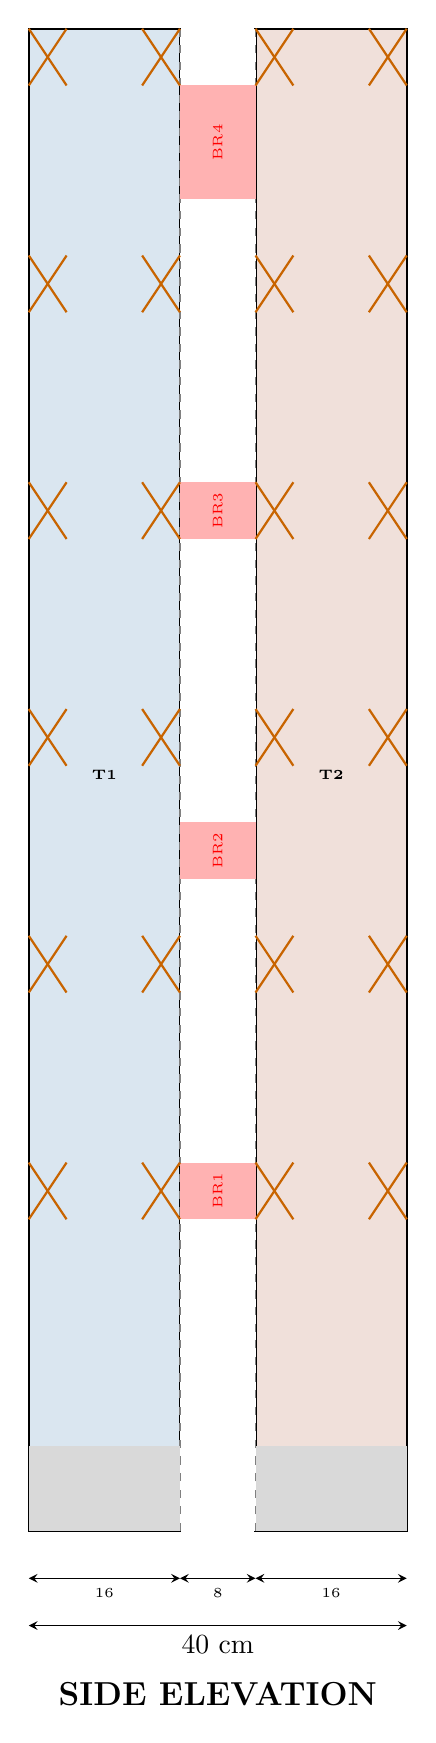
\begin{tikzpicture}[scale=0.12, font=\tiny]
    
    % Tower 1
    \draw[thick, fill=tower1!20] (0,0) rectangle (16, 159);
    
    % Tower 2
    \draw[thick, fill=tower2!20] (24,0) rectangle (40, 159);
    
    % Gap
    \fill[white] (16, 0) rectangle (24, 159);
    \draw[dashed, gray] (16, 0) -- (16, 159);
    \draw[dashed, gray] (24, 0) -- (24, 159);
    
    % Bridge zones
    \fill[red!30] (16, 33) rectangle (24, 39);
    \fill[red!30] (16, 69) rectangle (24, 75);
    \fill[red!30] (16, 105) rectangle (24, 111);
    \fill[red!30] (16, 141) rectangle (24, 153);
    
    \node[red, rotate=90] at (20, 36) {BR1};
    \node[red, rotate=90] at (20, 72) {BR2};
    \node[red, rotate=90] at (20, 108) {BR3};
    \node[red, rotate=90] at (20, 147) {BR4};
    
    % Mega-braces on side (every 4 floors)
    \foreach \f in {0, 4, 8, 12, 16, 20, 24} {
        \pgfmathsetmacro{\zbot}{(\f == 0) ? 0 : (\f * 6 + 9 - 24)}
        \pgfmathsetmacro{\zact}{\f * 6 + 9}
        \ifnum\f>0
            \draw[brace, thick] (0, \zact) -- (4, \zact + 6);
            \draw[brace, thick] (4, \zact) -- (0, \zact + 6);
            \draw[brace, thick] (12, \zact) -- (16, \zact + 6);
            \draw[brace, thick] (16, \zact) -- (12, \zact + 6);
            % Tower 2
            \draw[brace, thick] (24, \zact) -- (28, \zact + 6);
            \draw[brace, thick] (28, \zact) -- (24, \zact + 6);
            \draw[brace, thick] (36, \zact) -- (40, \zact + 6);
            \draw[brace, thick] (40, \zact) -- (36, \zact + 6);
        \fi
    }
    
    % Ground floor
    \fill[gray!30] (0, 0) rectangle (16, 9);
    \fill[gray!30] (24, 0) rectangle (40, 9);
    
    % Dimensions
    \draw[<->, >=stealth] (0, -5) -- (16, -5) node[midway, below] {16};
    \draw[<->, >=stealth] (16, -5) -- (24, -5) node[midway, below] {8};
    \draw[<->, >=stealth] (24, -5) -- (40, -5) node[midway, below] {16};
    \draw[<->, >=stealth] (0, -10) -- (40, -10) node[midway, below] {\normalsize 40 cm};
    
    % Labels
    \node at (8, 80) {\textbf{T1}};
    \node at (32, 80) {\textbf{T2}};
    \node[below] at (20, -15) {\large\textbf{SIDE ELEVATION}};
    
\end{tikzpicture}
\end{center}

\newpage

% ============================================================
% SECTION 3: TBDY2018 SPECTRUM (pgfplots)
% ============================================================
\section{TBDY2018 Design Spectrum}

\begin{center}
\begin{tikzpicture}
\begin{axis}[
    width=14cm,
    height=9cm,
    xlabel={Period $T$ (s)},
    ylabel={Spectral Acceleration $S_{ae}(T)$ (g)},
    title={\textbf{TBDY2018 Elastic Design Spectrum}},
    xmin=0, xmax=0.8,
    ymin=0, ymax=1.8,
    grid=both,
    grid style={line width=0.2pt, draw=gray!30},
    major grid style={line width=0.4pt, draw=gray!50},
    legend pos=north east,
    legend style={font=\small},
    tick label style={font=\small},
    label style={font=\normalsize},
    title style={font=\large},
]

% Spectrum data from TSV
\addplot[
    color=black,
    line width=1.5pt,
    mark=none,
] table[
    x=T,
    y=Sae,
    col sep=tab,
] {tbdy2018_spectrum.tsv};
\addlegendentry{TBDY2018 Spectrum}

% TA vertical line
\addplot[
    color=green!70!black,
    line width=1pt,
    dashed,
] coordinates {(0.0729, 0) (0.0729, 1.7)};
\addlegendentry{$T_A = 0.0729$ s}

% TB vertical line
\addplot[
    color=red!70!black,
    line width=1pt,
    dashed,
] coordinates {(0.3646, 0) (0.3646, 1.7)};
\addlegendentry{$T_B = 0.3646$ s}

% Current T1 point
\addplot[
    only marks,
    mark=*,
    mark size=4pt,
    color=red,
] coordinates {(0.0608, 1.401)};
\addlegendentry{$T_1 = 0.0608$ s}

% Annotation for T1
\node[anchor=south west, font=\small\bfseries, red, align=left] at (axis cs:0.08, 1.45) {
    $T_1 = 0.0608$ s, $S_{ae} = 1.401$ g
};

% Region labels
\node[font=\small, green!50!black] at (axis cs:0.035, 0.3) {Ascending};
\node[font=\small, red!70!black] at (axis cs:0.22, 0.3) {Plateau};
\node[font=\small, blue!70!black] at (axis cs:0.6, 0.3) {Descending};

\end{axis}
\end{tikzpicture}
\end{center}

\vspace{0.5cm}

\subsection{Spectrum Parameters}

\begin{center}
\begin{tabular}{|l|c|l|}
\hline
\textbf{Parameter} & \textbf{Value} & \textbf{Description} \\
\hline
$T_A$ & 0.0729 s & Ascending $\rightarrow$ Plateau transition \\
$T_B$ & 0.3646 s & Plateau $\rightarrow$ Descending transition \\
$S_{DS}$ & 1.556 g & Short period design spectral acceleration \\
\hline
$T_1$ & 0.0608 s & Fundamental period of structure \\
$S_{ae}(T_1)$ & 1.401 g & Spectral acceleration at $T_1$ \\
\hline
\end{tabular}
\end{center}

\subsection{Design Region}

\textbf{Current Status:} The structure is in the \textcolor{green!50!black}{\textbf{ASCENDING}} region ($T_1 < T_A$).

\begin{itemize}
    \item This is the optimal region for seismic design.
    \item Lower spectral acceleration compared to plateau region.
    \item Margin to $T_A$: $0.0729 - 0.0608 = 0.0121$ s (16.6\%)
\end{itemize}

\textbf{Warning:} Structures in the plateau region ($T_A \leq T \leq T_B$) experience maximum spectral acceleration, which can lead to critical design issues during earthquakes.

\newpage

% ============================================================
% SECTION 4: MODAL ANALYSIS RESULTS
% ============================================================
\section{Modal Analysis Results}

\subsection{Natural Periods (Mode 1-7)}

\begin{center}
\begin{tikzpicture}
\begin{axis}[
    width=12cm,
    height=7cm,
    ybar,
    bar width=0.6cm,
    xlabel={Mode Number},
    ylabel={Period $T$ (s)},
    title={\textbf{Modal Periods - OpenSeesPy Analysis}},
    symbolic x coords={1,2,3,4,5,6,7,8},
    xtick=data,
    ymin=0,
    ymax=0.08,
    nodes near coords,
    nodes near coords align={vertical},
    every node near coord/.append style={font=\tiny, rotate=90, anchor=west},
    grid=major,
    grid style={line width=0.2pt, draw=gray!30},
]

\addplot[fill=blue!60] table[
    x=Mode,
    y=Period,
    col sep=tab,
] {mode_periods_bar.tsv};

\end{axis}
\end{tikzpicture}
\end{center}

\subsection{Mode Shape - Mode 1 (X-Direction)}

\begin{center}
\begin{tikzpicture}
\begin{axis}[
    width=8cm,
    height=10cm,
    xlabel={Normalized Displacement $\phi_x$},
    ylabel={Height $z$ (m)},
    title={\textbf{Mode 1: $T_1 = 0.0608$ s}},
    xmin=-0.2, xmax=1.2,
    ymin=0, ymax=160,
    grid=both,
    grid style={line width=0.2pt, draw=gray!30},
]

\addplot[
    color=blue,
    line width=1.5pt,
    mark=*,
    mark size=2pt,
] table[
    x=phi_x,
    y=z,
    col sep=tab,
] {mode_shape_1.tsv};

\end{axis}
\end{tikzpicture}
\hspace{1cm}
\begin{tikzpicture}
\begin{axis}[
    width=8cm,
    height=10cm,
    xlabel={Normalized Displacement $\phi_x$},
    ylabel={Height $z$ (m)},
    title={\textbf{Mode 2: $T_2 = 0.0472$ s}},
    xmin=-1.2, xmax=1.2,
    ymin=0, ymax=160,
    grid=both,
    grid style={line width=0.2pt, draw=gray!30},
]

\addplot[
    color=red,
    line width=1.5pt,
    mark=*,
    mark size=2pt,
] table[
    x=phi_x,
    y=z,
    col sep=tab,
] {mode_shape_2.tsv};

\end{axis}
\end{tikzpicture}
\end{center}

\subsection{Mode Shapes - Modes 3 \& 4}

\begin{center}
\begin{tikzpicture}
\begin{axis}[
    width=8cm,
    height=10cm,
    xlabel={Normalized Displacement $\phi_x$},
    ylabel={Height $z$ (m)},
    title={\textbf{Mode 3: $T_3 = 0.0355$ s}},
    xmin=-1.2, xmax=1.2,
    ymin=0, ymax=160,
    grid=both,
    grid style={line width=0.2pt, draw=gray!30},
]

\addplot[
    color=green!70!black,
    line width=1.5pt,
    mark=*,
    mark size=2pt,
] table[
    x=phi_x,
    y=z,
    col sep=tab,
] {mode_shape_3.tsv};

\end{axis}
\end{tikzpicture}
\hspace{1cm}
\begin{tikzpicture}
\begin{axis}[
    width=8cm,
    height=10cm,
    xlabel={Normalized Displacement $\phi_x$},
    ylabel={Height $z$ (m)},
    title={\textbf{Mode 4: $T_4 = 0.0179$ s}},
    xmin=-1.2, xmax=1.2,
    ymin=0, ymax=160,
    grid=both,
    grid style={line width=0.2pt, draw=gray!30},
]

\addplot[
    color=orange,
    line width=1.5pt,
    mark=*,
    mark size=2pt,
] table[
    x=phi_x,
    y=z,
    col sep=tab,
] {mode_shape_4.tsv};

\end{axis}
\end{tikzpicture}
\end{center}

\subsection{Mode Shapes - Modes 5 \& 6}

\begin{center}
\begin{tikzpicture}
\begin{axis}[
    width=8cm,
    height=10cm,
    xlabel={Normalized Displacement $\phi_x$},
    ylabel={Height $z$ (m)},
    title={\textbf{Mode 5: $T_5 = 0.0119$ s}},
    xmin=-1.2, xmax=1.2,
    ymin=0, ymax=160,
    grid=both,
    grid style={line width=0.2pt, draw=gray!30},
]

\addplot[
    color=purple,
    line width=1.5pt,
    mark=*,
    mark size=2pt,
] table[
    x=phi_x,
    y=z,
    col sep=tab,
] {mode_shape_5.tsv};

\end{axis}
\end{tikzpicture}
\hspace{1cm}
\begin{tikzpicture}
\begin{axis}[
    width=8cm,
    height=10cm,
    xlabel={Normalized Displacement $\phi_x$},
    ylabel={Height $z$ (m)},
    title={\textbf{Mode 6: $T_6 = 0.0109$ s}},
    xmin=-1.2, xmax=1.2,
    ymin=0, ymax=160,
    grid=both,
    grid style={line width=0.2pt, draw=gray!30},
]

\addplot[
    color=cyan,
    line width=1.5pt,
    mark=*,
    mark size=2pt,
] table[
    x=phi_x,
    y=z,
    col sep=tab,
] {mode_shape_6.tsv};

\end{axis}
\end{tikzpicture}
\end{center}

\subsection{Mode Shapes - Modes 7 \& 8}

\begin{center}
\begin{tikzpicture}
\begin{axis}[
    width=8cm,
    height=10cm,
    xlabel={Normalized Displacement $\phi_x$},
    ylabel={Height $z$ (m)},
    title={\textbf{Mode 7: $T_7 = 0.0108$ s}},
    xmin=-1.2, xmax=1.2,
    ymin=0, ymax=160,
    grid=both,
    grid style={line width=0.2pt, draw=gray!30},
]

\addplot[
    color=brown,
    line width=1.5pt,
    mark=*,
    mark size=2pt,
] table[
    x=phi_x,
    y=z,
    col sep=tab,
] {mode_shape_7.tsv};

\end{axis}
\end{tikzpicture}
\hspace{1cm}
\begin{tikzpicture}
\begin{axis}[
    width=8cm,
    height=10cm,
    xlabel={Normalized Displacement $\phi_x$},
    ylabel={Height $z$ (m)},
    title={\textbf{Mode 8: $T_8 = 0.0096$ s}},
    xmin=-1.2, xmax=1.2,
    ymin=0, ymax=160,
    grid=both,
    grid style={line width=0.2pt, draw=gray!30},
]

\addplot[
    color=magenta,
    line width=1.5pt,
    mark=*,
    mark size=2pt,
] table[
    x=phi_x,
    y=z,
    col sep=tab,
] {mode_shape_8.tsv};

\end{axis}
\end{tikzpicture}
\end{center}

\subsection{Modal Analysis Summary}

\begin{center}
\begin{tabular}{|c|c|c|c|}
\hline
\textbf{Mode} & \textbf{Period (s)} & \textbf{Frequency (Hz)} & \textbf{Description} \\
\hline
1 & 0.0608 & 16.45 & 1st Translation (X) \\
2 & 0.0472 & 21.20 & 1st Translation (Y) \\
3 & 0.0355 & 28.15 & 1st Torsion \\
4 & 0.0179 & 55.88 & 2nd Translation \\
5 & 0.0119 & 84.23 & Higher Mode \\
6 & 0.0109 & 91.69 & Higher Mode \\
7 & 0.0108 & 92.28 & Higher Mode \\
8 & 0.0096 & 104.69 & Higher Mode \\
\hline
\end{tabular}
\end{center}

\vspace{0.5cm}

\textbf{Analysis Parameters:}
\begin{itemize}
    \item Software: OpenSeesPy (Python)
    \item Material: Balsa Wood ($E = 3500$ MPa, $\rho = 160$ kg/m$^3$)
    \item Section: $6 \times 6$ mm
    \item Total Mass: 15.02 kg (test loads at every 3 floors)
\end{itemize}

\end{document}
